%!TEX root = ../thesis.tex
%*******************************************************************************
%****************************** Third Chapter **********************************
%*******************************************************************************

% **************************** Define Graphics Path **************************

\ifpdf
    \graphicspath{{Chapter2/Figs/Raster/}{Chapter2/Figs/PDF/}{Chapter2/Figs/}}
\else
    \graphicspath{{Chapter2/Figs/Vector/}{Chapter2/Figs/}}
\fi

%\ref{sec:reactorAntiNeutrinos}

\chapter{Overview of Neutrino Physics}\label{Chp:ABfriefHistoryOfNeutrinos} 
To illustrate the nature and unique properties of the neutrino a historical look at the discovery of the neutrino will be used in this chapter. This will include the proposal of the neutrino to solve the missing energy in beta decay and the more direct observations in emulsion, as well as an overview of how lepton number and flavour impacted the understanding of the neutrino physics. Then the experimental evidence and theory behind neutrino oscillation will be covered. Finally, how neutrino oscillation might effect reactor neutrino monitoring will be explored. %And the impact of neutrino oscillations on neutrinos and the impact of oscillations on reactor measurements. 

\section{Theoretical Development}
%history of neutrino: \cite{griffiths2008neutrino1.5} \cite{lederman1970resource}
%\\beta decay of tritium (book cannot find, may have to replicate): \cite{lewis1970neutrinos} especially as Fermi mentions it in \cite{Fermi:1934hr}, \cite{wilson1968fermi} 
%\\Neutron proposed by Chadwick in 1932 describing a proton like recoil and odd behaviour of neutrons that can only be described by a neutron or the breaking of conservation of momentum and energy!: \cite{chadwick1932possible}. Important for giving full context to the neutrino discovery
%\\Fermis paper proposing this beta decay after Chadwick's discovery of the neutron is given in \cite{Fermi:1934hr} which proposes a neutrino and is published through Springer and the English translation from 1968 is given in \cite{wilson1968fermi}
%\\So far very little from Pauli need to include him somewhere the neutrino was his idea \cite{lederman1970resource} may have something...
The neutrino was postulated by Pauli in 1931 as a way to conserve both the energy of beta decay and the angular momentum of the products of beta decay  \cite{griffiths2008neutrino1.5}\cite{lederman1970resource}. At the time beta decay was described by equation \ref{oldBetaDecay}. Where $A$ and $B$ represent the decaying particles, as the neutron had not yet been discovered by this point, it was considered a reaction between two nuclei. The conservation of energy dictates that the kinetic energy of the electron should only have a discrete value as shown in equation \ref{constant_ke_e_equation}. However, when the kinetic energy of the electron was measured (see figure \ref{fig:beta_spectrum}) the energy of the electron formed a continuum as seen in figure \ref{fig:beta_spectrum}  \cite{griffiths2008neutrino1.5} \cite{lewis1970neutrinos}. Equation \ref{constant_ke_e_equation} represents the maximum possible energy available to the electron in figure \ref{fig:beta_spectrum} suggesting a third body in beta decay  \cite{griffiths2008neutrino1.5}.


\begin{equation}
    A \rightarrow B + e^-
    \label{oldBetaDecay}
\end{equation}

\begin{equation}
    E = \left( \frac{{m_A}^2 - {m_B}^2 + {m_e}^2}{2m_A}\right) c^2
    \label{constant_ke_e_equation}
\end{equation}

\begin{figure}[!h]
 \centering
 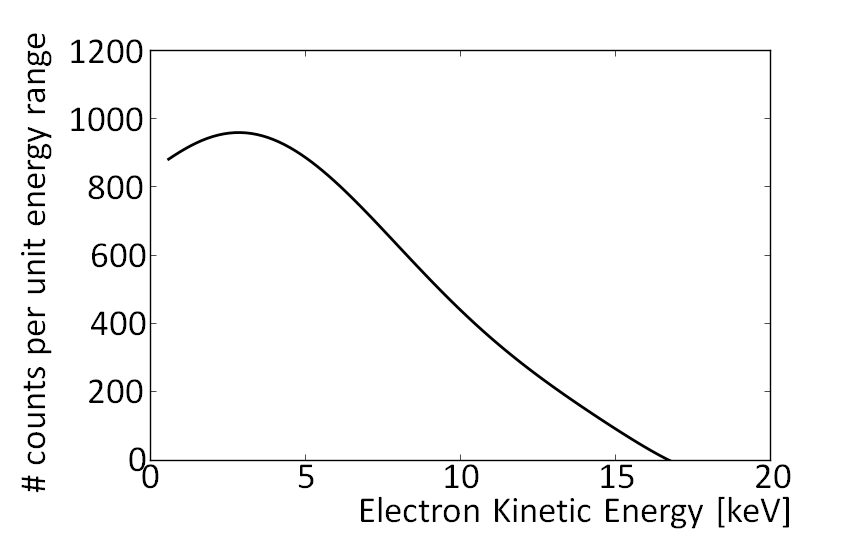
\includegraphics[width=0.7\linewidth]{Chapter1/Figs/Raster/betaSpectrum.png}
 \captionof{figure}{beta spectrum reproduced from \cite{griffiths2008neutrino1.5} originally from \cite{lewis1970neutrinos}. The energy of the $e^-$ from beta decay varies significantly suggesting a 3 body decay model for beta decay instead of a 2 body model.} %~can be used as a kind of place holder in latex
 \label{fig:beta_spectrum}
\end{figure}

The beta spectrum shown in figure \ref{fig:beta_spectrum} was the first indirect evidence that neutrinos may exist. However, Pauli waited until Chadwick's discovery of the neutron in 1932 \cite{chadwick1932possible} before publishing in 1934 \cite{lederman1970resource}. The complete picture of a proton-neutron nucleus allowed Enrico Fermi to formulate a comprehensive theory of beta decay which incorporated Pauli's neutrino into beta decay\footnote{a translation of Fermi's work was used \cite{wilson1968fermi}} \cite{lederman1970resource} \cite{Fermi:1934hr}. This more complete picture made sure to differentiate the particles of the nucleus (protons and neutrons) from particles that were not bound to it (electrons and neutrinos) \cite{Fermi:1934hr} \cite{wilson1968fermi}. However, this results in a massless neutrino \cite{lederman1970resource}. The discovery of neutrino oscillations (mentioned later in section \ref{section_neutrino_oscillations}) indicates that neutrinos do have mass, but oscillations were discovered long after this  \cite{griffiths2008neutrino1.5}. The more complete picture as illustrated by equation \ref{semi_modern_beta_decay} by Fermi now integrated the neutrino. The discovery of lepton number and $\Bar{\nu}$ had not yet been made and so that quantity is not conserved in equation \ref{semi_modern_beta_decay}. 

\begin{equation}
    n \rightarrow p^+ + e^- + \nu
    \label{semi_modern_beta_decay}
\end{equation}

\section{Direct Measurements}\label{Direct_Measurements_section}
%propossal of cowan and riens using a large liquid scintillator detector: \cite{reines1953proposed}
%\\First detection: \cite{reines1953detection}
%\\distingiusing the neutrino and anti-neutrino \cite{davis1959attempt}
%\\Need to find cloud chamber pictures showing the conservation of momentum  \cite{griffiths2008neutrino1.5} shows them, need to find direct source.  \cite{griffiths2008neutrino1.5} also goes on to explain why this matters.
%\\ \cite{michel1949energy} supposedly does show this, but I'm having trouble getting my hands on it, UoL doesn't have access to nature papers! So will just have to include a picture from  \cite{griffiths2008neutrino1.5} and clarifiy it is from \cite{michel1949energy}.
%\\ There is also the suggestion from cowan early on that anti-neutrinos and neutrinos are differing particles,  \cite{cowan1957test}, however this is by no means certain it is possible that neutrinos and anti-neutrinos are differing spin states of the same particle.
%\\ There is also the early suggestion of neutrinos and anti neutrinos being separated by a certain quantity suggested by \cite{konopinski1953universal} under a universal interaction. They use $\mu$ to suggest that certain reactions are not possible, this would later come to be known as lepton number. \\\\
%Suggestions of differing types of neutrino supposedly come from the Soviet union in 1960 but this has been lost to the iron curtain unfortunately I could not find the paper myself. The earliest reference I found is \cite{pontecorvo1963neutrino} in 1963 talking about how this influences astrophysics. 
%\\The direct measurement of differing types of neutrinos was done by \cite{DanbyG1962PhysRevLett.9.36} in 1962. This was done with a pion beam striking a beryllium target and a 10 ton spark chamber behind the target in order to pick up 37 events of one reaction and not another. They also make reference to kions but seem less certain about those due to experimental limitations. They call this the ``The neutrino flip hypothesis.'' This is a really important paper.\\

Experimental evidence for a neutrino had been observed as early as 1949, in figure \ref{pion_path} it is possible to see the change in direction due to the neutrino: the neutrino itself is neutral and so leaves no track in the emulsion. However, the effect of the neutrino can be seen when the anti-pion ($\pi^-$) decays into a muon ($\mu^-$) and when the muon decays into an electron ($e^-$)  \cite{griffiths2008neutrino1.5}. Collisions in the emulsion cannot account for the 90$^\circ$ change in direction as the particles decay. Collisions can only account for dithering but not the abrupt changes in direction  \cite{griffiths2008neutrino1.5}. At the time it was practical to assume that the pion decay shown in equation \ref{pion_nolepNo_decay} and the muon decay shown in equation \ref{muon_nolepNo_decay} both produced the same particle when decaying, the neutrino ($\nu$)  \cite{griffiths2008neutrino1.5}. However, as seen in equations \ref{pion_nolepNo_decay} and \ref{muon_nolepNo_decay}, lepton number and neutrino flavour were not yet known and and so are not present in equations \ref{pion_nolepNo_decay} and \ref{muon_nolepNo_decay}.
\begin{equation}
    \pi^- \rightarrow \mu^- + \nu^-
    \label{pion_nolepNo_decay}
\end{equation}
\begin{equation}
    \mu^- \rightarrow e^- + 2\nu
    \label{muon_nolepNo_decay}
\end{equation}
\\
\begin{figure}[!h]
 \centering
 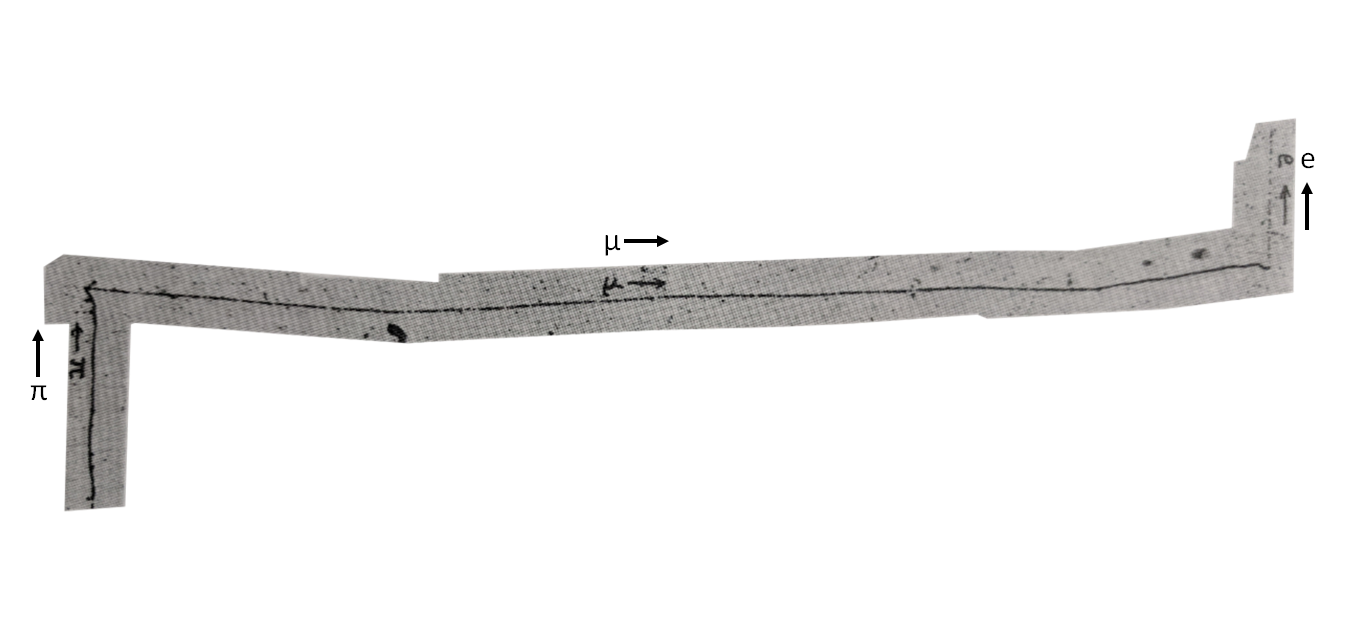
\includegraphics[width=0.8\linewidth]{Chapter1/Figs/Raster/neutrinoInChamberRotated90.png}
 \captionof{figure}{Path of a anti-pion decaying to a muon emitting one anti-neutrino (equation \ref{pion_nolepNo_decay}) and then that muon decaying into an electron-emitting a neutrino and an anti-neutrino (equation \ref{muon_nolepNo_decay}). The paths at 90$^o$ show particle decay, collisions cannot account for this. From \cite{griffiths2008neutrino1.5} originally published in \cite{michel1949energy}.} %~can be used as a kind of place holder in latex
 \label{pion_path}
\end{figure}
\\The first direct detection of a neutrino would be 22 years after it was proposed in 1931. In 1953, Cowan and Reines proposed a neutrino detector that used a large amount of liquid scintillator to detect neutrinos \cite{reines1953proposed}. Later that same year they constructed a cadmium loaded scintillation detector that used a delayed coincidence measurement of IBD to reduce background \cite{reines1953proposed} \cite{reines1953detection} (result mentioned in section \ref{sec:reactorAntiNeutrinos}). The measurement of neutrino candidates was later reproduced with greater accuracy in 1956 at the Savannah River Plant \cite{Cowan1956Confirmation}. This new detector used a combination of liquid scintillator in three layers and cadmium chloride doped water in another two layers in a ``club-sandwich'' arrangement \cite{Cowan1956Confirmation}. This resulted in an unambiguous measurement of 0.56 $\pm$ 0.06 counts per hour with a signal 20 times higher than the accidental background associated with the reactor \cite{Cowan1956Confirmation}. The delayed coincidence technique assumed $\sim$ 5$\mathrm{\mu}$s between the prompt positron signal and the delayed neutron signal \cite{reines1953detection}. This approach was so successful that its used to this day in many other detector experiments (including the VIDARR detector).
\\\\The difference between neutrinos and anti-neutrinos or their flavours was not yet known. There were two possible hypotheses: Majorana neutrinos where the neutrino and the anti-neutrino are the same particle, and Dirac neutrinos where they are distinct particles  \cite{griffiths2008neutrino1.5} \cite{cowan1957test}. The possibility of Majorana neutrinos was questioned as measurements of double beta decay were found to conflict with the Majorana hypothesis \cite{cowan1957test}. The lifetime of such a particle would be too short compared to measurements made of beta decay \cite{cowan1957test}. A direct attempt at measuring the difference between neutrinos and anti-neutrinos was made in 1959 \cite{davis1959attempt}. The Homestake Mine experiment relied on using $^{37}$Cl and then measuring the amount of $^{37}$Ar produced (equation \ref{neutrino_chlorine_decay}) \cite{davis1959attempt}. From previous experiments the interaction between a neutron and a neutrino (equation \ref{no_lepNo_dirac_nu_capture}) was known to occur \cite{Cowan1956Confirmation}. But whether the anti-neutrino would also act in the same manner (equation \ref{no_lepNo_maj_nu_capture}) was not known. If anti-neutrinos did not act as neutrinos then the Majorana hypothesis was unlikely as neutrinos and anti-neutrinos were probably distinct particles  \cite{griffiths2008neutrino1.5} \cite{davis1959attempt}. Candidates for anti-neutrinos acting as neutrinos (equation \ref{no_lepNo_maj_nu_capture}) were observed 20 times below what would be expected for the Majorana hypothesis \cite{davis1959attempt}. Therefore, Dirac neutrinos were considered to be more consistent with the experiment (though this does not strictly disprove the Majorana hypothesis \cite{griffiths2008neutrino1.5} and searches for neutrino-less double beta decay are ongoing to this day). 
\begin{equation}
    \nu_e + ^{37}Cl \rightarrow  e^- + ^{37}Ar
    \label{neutrino_chlorine_decay}
\end{equation}
\begin{equation}
    n + \nu \rightarrow p^+ + e^-
    \label{no_lepNo_dirac_nu_capture}
\end{equation}
\begin{equation}
    n + \Bar{\nu} \rightarrow p^+ + e^-
    \label{no_lepNo_maj_nu_capture}
\end{equation}
\\This experimental result had been predicted years prior by \cite{konopinski1953universal} which proposed a ``universal interaction'' for ``light'' and ``heavy'' particles. An undetermined phase factor c was represented as $c_P=c_N=c_H$ and $c_e=c_\mu=c_\nu=c_L$ where L and H stand ``light'' and ``heavy'' respectively. In addition to this the muon decays were suggested to give out two differing types of neutrino (equation \ref{noLep_dirac_mu_decay})  \cite{griffiths2008neutrino1.5}, \cite{konopinski1953universal}. Both of these observations would later be consolidated into a quantity known as lepton number with $L=+1$ for electrons, muons and neutrinos but $L=-1$ for positrons, anti-muons and anti-neutrinos \cite{griffiths2008neutrino1.5}. 
\begin{equation}
    \mu^- \rightarrow e^- + \nu + \Bar{\nu}
    \label{noLep_dirac_mu_decay}
\end{equation}
\\However, the conservation of flavours was not yet known hence the lack of neutrino flavours when describing muon decay (equation \ref{noLep_dirac_mu_decay})  \cite{griffiths2008neutrino1.5}. There were hints that flavour conservation was necessary as muon decay into an electron with no neutrinos (equation \ref{mu_forbiden_decay}) was never observed \cite{griffiths2008neutrino1.5}. When a muon decays into an electron two neutrinos must be emitted (equation \ref{noLep_dirac_mu_decay}). The sharp 90$^\circ$ changes in direction with no other particles visible in the emulsion seen in figure \ref{pion_path} strongly suggest neutrino emission. This led to the suggestion that the neutrinos emitted by the decay of muon into electrons were of different types i.e. neutrinos are not anti-neutrinos \cite{Lee:1960tja}  \cite{griffiths2008neutrino1.5}. Thus, redefining lepton numbers to include flavours such that: $L_{e^-} = +1$, $L_e^+ = -1$, $L_{\mu^-} = +1 $, $L_{\mu^+} = -1 $. With this understanding, equation \ref{noLep_dirac_mu_decay} became equation \ref{proper_mu_decay}.
\begin{equation}
    \mu^- \not\to e^- + \gamma
    \label{mu_forbiden_decay}
\end{equation}
\begin{equation}
    \mu^- \rightarrow e^- + \nu_\mu + \Bar{\nu}_e
    \label{proper_mu_decay}
\end{equation}
\\An experiment to measure the different types of neutrinos was then performed in 1962 \cite{DanbyG1962PhysRevLett.9.36}. This experiment used a pion beam striking a beryllium target and ten 1-ton spark chambers to measure the results. If electron anti-neutrinos and muon anti-neutrinos are the same particle then the production of electrons (equation \ref{test_e_decay}) and the production of muons (equation \ref{test_mu_decay}) should occur at equal rates \cite{DanbyG1962PhysRevLett.9.36}:
\begin{equation}
    \begin{split}
    \nu + n \rightarrow p + e^- \\
    \Bar{\nu} + p \rightarrow n + e^+
    \label{test_e_decay}
    \end{split}
\end{equation}
\begin{equation}
    \begin{split}
    \nu + n \rightarrow p + \mu^-  \\
    \Bar{\nu} + p \rightarrow n + \mu^+
    \label{test_mu_decay}
    \end{split}
\end{equation}
The neutrino ``beam'' used produced 34 muons in the spark chambers 5 of which were considered to be background due to cosmic rays. Therefore $\sim$ 29 electron events were expected to be produced if electron neutrinos and muon neutrinos were the same particle however only 6 candidates were identified \cite{DanbyG1962PhysRevLett.9.36}. To further prove that they were not the same particle two of the 1-ton spark chambers were tested at the electron beams at the Cosmotron, a GeV scale synchrotron, which did produce electrons similar to what would have been expected if they were the same particle. The events from the Cosmotron data set looked very different from the 6 candidate reactions observed from the pion beam being described as ``showers of qualitatively different appearance'' by Danby et. al. \cite{DanbyG1962PhysRevLett.9.36}. The interpretation that electron anti-neutrinos were not muon anti-neutrinos was the most likely conclusion, meaning that there were at least two different flavours of neutrinos \cite{DanbyG1962PhysRevLett.9.36}. And with this information, the modern form of beta decay is shown by equation \ref{modern_beta_decay}.
\begin{equation}
    n \rightarrow p + e^- + \Bar{\nu_e} 
    \label{modern_beta_decay}
\end{equation}

\section{Experimental Evidence For Neutrino Oscillation}\label{sec:neutrinoFlavours}
In the Standard Model it is easier for the neutrino to be assumed as massless, though there is no fundamental reason for neutrinos to be massless, it simplifies much in the standard model if this is the case \cite{griffiths2008neutrinoOscillations}. However, this assumption though simple and neat is now known to be wrong. In particular, the phenomena of neutrino oscillation where neutrinos oscillate between different mass and flavour states proves that neutrinos cannot be massless \cite{griffiths2008neutrinoOscillations}. The first experimental evidence of neutrino oscillations was the solar neutrino problem where the predicted rate by the Standard Solar Model (SSM) by Bahcall in 1968 did not match the measured rate from the previously mentioned Homestake Mine experiment \cite{griffiths2008neutrinoOscillations}. Bahcall attempted to model the expected neutrino rate for the $^{37}$Cl the predicted rate was $3.5 \times 10 ^{-35} \ \textrm{sec}^{-1} \ \textrm{per} \ ^{37}\textrm{Cl} \ \textrm{atom}$ \cite{bahcall1968present}. This conflicted with the measured result from the Homestake Mine of 2.0 $\pm$ 1.2 $\times$ 10 $^{-35}$ sec$^{-1}$ per $^{37}$Cl atom \cite{davis1968homestake}. At the time the large uncertainty on each of these predictions provided some possibility of reconciliation. 
\\\\However, as the Homestake experiment continued to take measurements a discrepancy of about one third became more pronounced over time \cite{griffiths2008neutrinoOscillations}. The Homestake experiment continued to take data until 1995 and produced the result $\Phi$Cl = 2.56 $\pm$ 0.16 Solar Neutrino Unit (SNU) \cite{Bellerive:2003rj}. The SSM continued to be improved and the predicted rate for $\Phi$Cl was 7.6$^{+ 1.3}_{-1.1}$ SNU \cite{Bellerive:2003rj}. But chlorine is not the only way in which neutrinos can be measured. The Sudbury Neutrino Observatory (SNO) used heavy water to measure neutrino interaction and the Kamiokande and later Super-Kamiokande (SuperK) experiments would use normal water to measure neutrino interactions \cite{Bellerive:2003rj}. These experiments are sensitive to different parts of the solar neutrino spectrum with SuperK and SNO being more sensitive to higher energies than the chlorine experiments \cite{Bellerive:2003rj}. The SuperK experiment used neutrino scattering to detect any type of neutrino but is 6.5 times more sensitive to electron neutrinos \cite{griffiths2008neutrinoOscillations}. SNO also works through neutrino scattering but also works through the charged-current (CC) interaction and  the neutral-current (NC) interaction) \cite{sno2001}\cite{Bellerive:2003rj} \cite{griffiths2008neutrinoOscillations}. 
\\\\By combining the results from SuperK which uses exclusively neutrino scattering and the SNO results for CC it is possible to solve the solar neutrino problem. SuperK found 45.1\,\% $\pm$ 0.5\,\% (stat)$^{+1.6\,\%}_{-1.4\,\%}$ (syst) according to the BP2000 standard solar model \cite{superK2001}. Whereas the CC interaction results from SNO found 34.7\,\% $\pm$ 2.9\,\% of the expected electron neutrino flux\cite{sno2001}. There is a $\sim$ 10\,\% discrepancy between these two results. But this does not mean 10\,\% of the neutrinos were muon neutrinos and tau neutrinos, as the SuperK detector is 6.5 times more sensitive to electron neutrinos. 10\,\% $\times$ 6.5 = 65\,\%, therefore 65\,\% of the neutrinos are muon and tau flavoured neutrinos. And so all neutrinos are now accounted for as the Cl results from SNO accounted for the other 35\,\% and thus the solar neutrino problem was deemed solved  \cite{griffiths2008neutrinoOscillations}. The results showed that neutrino oscillations had a clear experimental basis for their existence proving that the solar neutrinos were changing flavours as they traversed through space. 
\\\\In addition, atmospheric neutrino oscillation has also been observed. Atmospheric neutrino production is dominated by production from equations \ref{equ:pi+AtmosNu} and \ref{equ:mu+AtmosNu} (and their charge conjugates):
\begin{equation}
    \pi^+ \rightarrow \mu^+ + \nu_\mu
    \label{equ:pi+AtmosNu}
\end{equation}
\begin{equation}
    \mu^+ \rightarrow e^+ + \Bar{\nu_\mu} + \nu_e
    \label{equ:mu+AtmosNu}
\end{equation}
This gives an expected ratio of muon neutrinos and muon anti-neutrinos to electron neutrinos and electron anti-neutrinos of $\sim$ 2 (equation \ref{equ:ratioAtmosNu}) \cite{fukuda_skAtmosAnnounce_1998}:
\begin{equation}
    R_{\textrm{data}/\textrm{MC}} = (N_\mu/N_e)_{\textrm{data}}/(N_\mu/N_e)_{\textrm{MC}} \approx 2
    \label{equ:ratioAtmosNu}
\end{equation}
But instead more equal numbers were found \cite{fukuda_skAtmosAnnounce_1998} \cite{KAJITA_sk_atmospheric_2016}. Atmospheric neutrino disappearance was found in the IMB detector in 1986 \cite{tjHaines_AtmosModel_1986} and was also observed in SuperK in 1988 \cite{Hirata_sk_atmosStudy_1988} \cite{KAJITA_sk_atmospheric_2016}. By 1986 and 1988 the theory of oscillations was quite well known and this was suggested in 1986 as a possible explanation \cite{tjHaines_AtmosModel_1986}. But it took until 1998 when SuperK calculated an R$_{\textrm{data}/\textrm{MC}}$ value of $\sim = 0.63 - 0.65$, depending on energy range \cite{fukuda_skAtmosAnnounce_1998}. 
\\\\These results show how the theory of neutrino oscillations has strong experimental backing. This is important as the simplest scenario of massless neutrinos cannot explain the results of atmospheric and solar neutrino disappearance and reappearance that oscillations can. And as such this subsequent rejection of massless neutrinos and strong favouring of neutrino oscillations highlights why the theory of oscillations needs to be considered for any neutrino experiment. 

% \section{Solar Neutrinos}
% %This section will mainly be on the solar neutrino problem and how it was solved. The main players here are the homestake %experiment for detecting a certain number of neutrinos  \cite{davis1968homestake}. Bahcall for predicting three times more %solar neutrinos than were detected from that experiment \cite{bahcall1968present}. As well as the Kamiokande-II experiment %which made measurements in 1989 \cite{Kamiokande-II1989} which predicted $\sim$ 0.46 times the predicted $\nu$ flux from %the sun. And then finally the SNO and superK experiments in 2001 which are considered the final confirmation. SuperK %reference being \cite{superK2001}. And \cite{sno2001} for SNO.
% %\\This section may also be well served by explaining the proton-proton chain briefly as well as mentioning the CNO cycle %that isn't the power mechanism for our sun, if only because the 1968 papers mention it. Also figure out how to do sub %references for  \cite{griffiths2008neutrinoOscillations}. 
% %\\ \cite{Bellerive:2003rj} presents some good plots and a nice overview of the neutrino experiments that lead up to the %discovery of the neutrino oscillations. A nice overview.
% Whilst the neutrino flavous were being confirmed \cite{DanbyG1962PhysRevLett.9.36} preperations to measure the solar neutrino flux were also underway. The first measurement in the Homestake mine in 1968 found 31 $\pm$ 10 neutrinos from the sun \cite{davis1968homestake} by using $^{37}$Cl which interacts with $\nu_e$ as shown in equation \ref{neutrino_chlorine_decay} \cite{Bellerive:2003rj}. Which measured the production of $\nu_e$ from $^8$B interactions in the sun ($^8$B neutrino production is preferred due to the higher energy of neutrinos produced \cite{griffiths2008neutrinoOscillations}). Originally, this measurement was attempting to conclude whether the CNO cycle played a significant role in the sun's power production, concluding that it was less than 9\% of the power produced \cite{davis1968homestake}. However, when Bahcall attempted to model the expected neutrino rate for the $^{37}$Cl the predicted rate was 3.5 $\times$ 10 $^{-35}$ sec$^{-1}$ per $^{37}$Cl atom. Which conflicted with the measured result from the Homestake mine of 2.0 $\pm$ 1.2 $\times$ 10 $^{-35}$ sec$^{-1}$ per $^{37}$Cl atom \cite{davis1968homestake}. This is considered to be the birth of the solar neutrino problem \cite{griffiths2008neutrinoOscillations}. But it is worth pointing out this is somewhat of a retroactive view. At the time it was hoped that these discrepancies would be resolved as the errors were significant. In fact the prediction paper concluded ``...there is no irreconcilable discrepancy between our predictions and the experiment of Davis, Harmer, and Hoffman when the uncertainties in the various parameters that enter the calculation are taken into account'' \cite{bahcall1968present}.
% \\\\However, as the Homestake experiment continued to run a discrepancy of $\sim 1/3$ became more pronounced over time \cite{griffiths2008neutrinoOscillations}. The Homestake experiment continued to take data until 1995 and produced the result $\Phi$Cl = 2.56 $\pm$ 0.16 Solar Neutrino Unit (SNU) \cite{Bellerive:2003rj}. The standard solar model (SSM) continued to be improved and the predicted rate for $\Phi$Cl was 7.6$^{+ 1.3}_{-1.1}$ SNU \cite{Bellerive:2003rj}. However, chlorine is not the only way in which neutrinos can be measured the Sudbury Neutrino Observatory (SNO) used heavy water to measure neutrino interaction and the Kamiokande and later SuperKamiokande (SuperK) experiments would use normal water to measure neutrino interactions \cite{Bellerive:2003rj}. These experiments are sensitive to different parts of the solar neutrino spectrum as seen in figure \ref{neutrino_emmision_graph} with SuperK and SNO being more sensitive to higher energies than the chlorine experiments. The SuperK experiment used neutrino scattering (equation \ref{neutrino_scattering}) to detect any type of neutrino but is 6.5 times more sensitive to electron neutrinos  \cite{griffiths2008neutrinoOscillations}. SNO also works through neutrino scattering but also works through the charged-current (CC) reaction (equation \ref{charged-current_reaction}) and  the neutral-current (NC) reaction (equation \ref{neutral-current_reaction}) \cite{sno2001}\cite{Bellerive:2003rj}  \cite{griffiths2008neutrinoOscillations}. 
% \begin{figure}[!h]
%  \centering
%  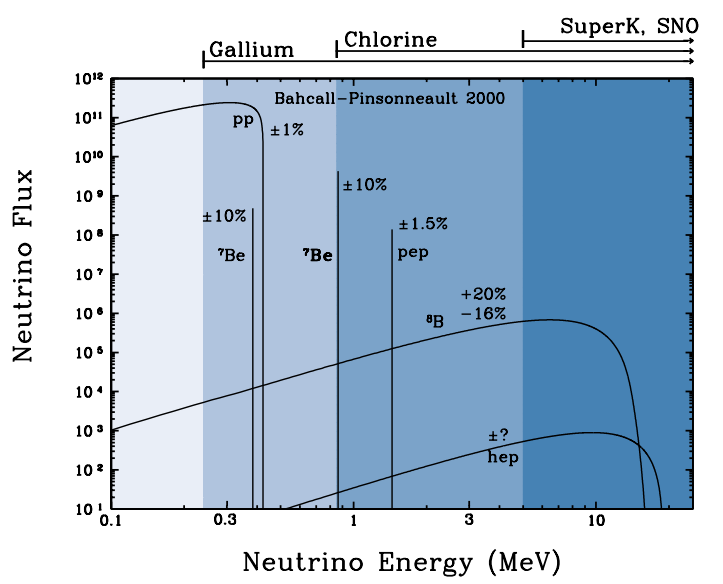
\includegraphics[width=0.7\linewidth]{Chapter1/Figs/Raster/neutrino_emmision_graph.png}
%  \captionof{figure}{The solar neutrino spectra predicted by the SSM. From \cite{Bellerive:2003rj}. The neutrino fluxes at one astronomical unit from continuum sources are given in units of cm$^{-2}$ s$^{-1}$ MeV$^{-1}$ , and the line fluxes are given in cm$^{-2}$ s$^{-1}$.} %~can be used as a kind of place holder in latex
%  \label{neutrino_emmision_graph}
% \end{figure}
% \begin{equation}
%     \nu + e \rightarrow  \nu + e
%     \label{neutrino_scattering}
% \end{equation}
% \begin{equation}
%     \nu_e + d \rightarrow p + p + e 
%     \label{charged-current_reaction}
% \end{equation}
% \begin{equation}
%     \nu + d \rightarrow  n + p + \nu
%     \label{neutral-current_reaction}
% \end{equation}
% \\By combining the results from SuperK which uses exclusively neutrino scattering and the SNO results for CC it is possible to solve the solar neutrino problem. SuperK found 45.1\,\% $\pm$ 0.5\,\% (stat)$^{+1.6\,\%}_{-1.4\,\%}$ (syst) according to the BP2000 standard solar model \cite{superK2001}. Whereas the CC results from SNO found 34.7\,\% $\pm$ 2.9\,\% of the $\nu_e$ expected as seen in figure \ref{sno_superK_comparision_plot} \cite{sno2001}. There is a $\sim$ 10\,\% discrepancy between these two results. But this does not mean 10\,\% of the neutrinos were $\nu_\mu$ and $\nu_\tau$, as the SuperK detector is 6.5 times more sensitive to $\nu_e$. 10\,\% $\times$ 6.5 = 65\,\%, therefore 65\,\% of the neutrinos are $\nu_\mu$ and $\nu_\tau$. And so all neutrinos are now accounted for as the Cl results from SNO accounted for the other 35\,\% and thus the solar neutrino problem was deemed solved  \cite{griffiths2008neutrinoOscillations}. The result was that neutrino oscillations had a clear experimental basis for their existence. As it was clear that the solar neutrinos were changing flavours as they traversed through space. 

% %\cite{Ashenfelter:2015tpm} %prospect citation

% \begin{figure}[!h]
%  \centering
%  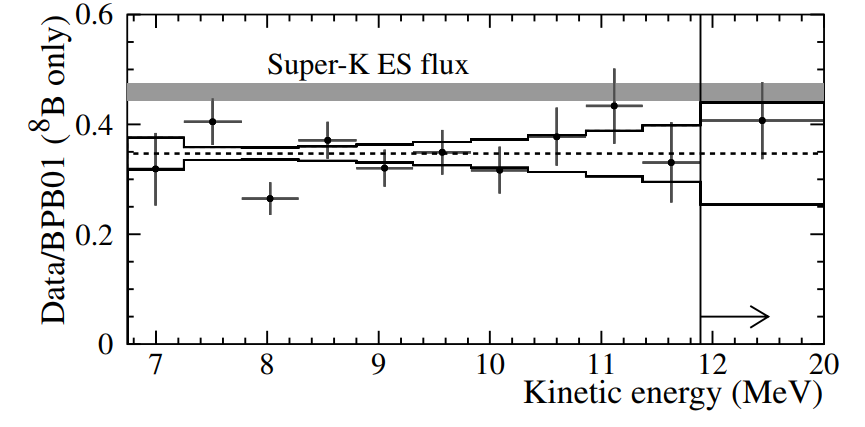
\includegraphics[width=0.7\linewidth]{Chapter1/Figs/Raster/superKSnoComparison.png} %height of this plot had to be adjusted because of its unusal diemensions
%  \captionof{figure}{The ratio of the data to the expected kinetic energy distribution with correlated systematic errors for the $^8$B charged current interactions. Notice the $\sim$ 10 \,\% discrepancy in data between the super K elastic scattering flux (in shaded grey) and the SNO charged current flux (the dashed line). From \cite{sno2001}.} %~can be used as a kind of place holder in latex
%  \label{sno_superK_comparision_plot}
% \end{figure}


% %\begin{figure}[!h]
% % \centering
% % 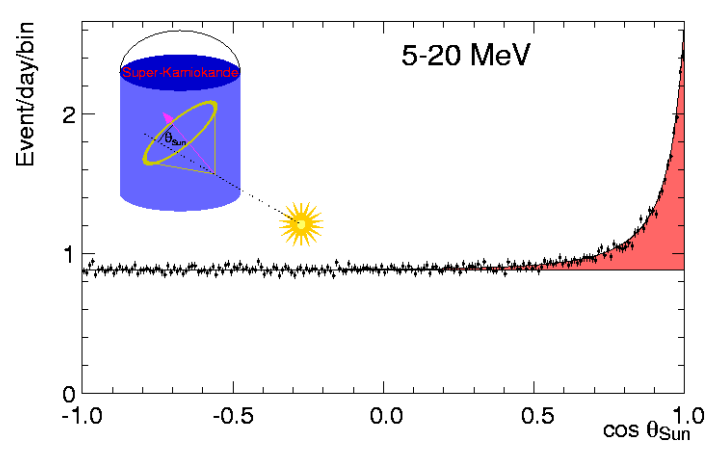
\includegraphics[height=90mm]{sk_angular_neutrinos.png}
% % \captionof{figure}{from \cite{Bellerive:2003rj}} %~can be used as a kind of place holder in latex
% % \label{sk_angular_neutrinos}
% %\end{figure}

\section{Two Neutrino Oscillation Theory} \label{section_neutrino_oscillations}
% Neutrino oscillations were proposed in 1968 after the Davis experiment \cite{davis1968homestake}. A man called Pontecorvo discussed the possibility of oscillations in 1957 and revived the idea in 1968 as a solution to the solar neutrino problem \cite{griffiths2008neutrinoOscillations}. With the original 1958 paper being \cite{pontecorvo1958_OscillationProposal}, suggesting the transformation of Kiaons. And the suggestion for the solution to the solar neutrino problem being here \cite{pontecorvo_gibov_1969_solar_oscillation}. Note these are a little hard to get hold of but some old russian servers still have them, Googling not too hard. 
% \\Most of this section will follow  \cite{griffiths2008neutrinoOscillations}. There is a more in depth explanation using \cite{sassaroli1999neutrino} in which  \cite{griffiths2008neutrinoOscillations} follows the standard treatment for neutrino oscillations. \cite{sassaroli1999neutrino} also goes through a relativistic treatment but that's probably too much for this overview and not really necessary for explaining the phenomena of oscillations, it should still be mentioned though. Wavelength of neutrino and kaon oscillations mentioned before are outlined by \cite{burkhardt2003wavelength}, it goes through the kinematics and shows that the oscillations do account for the mass difference, again quite in depth maybe overkill... should talk to one of my supervisors about this... 
% \\Also there is the MSW (named after the people who found it) effect however the exact papers appear to be a bit difficult to find but I was able to get something very detailed from Mikheev 1987 which goes into interactions with matter \cite{Mikheev_1987}.
Neutrino oscillations had been proposed in 1958 by Pontecorvo by analogy with $K^0$/$\Bar{K^0}$   \cite{griffiths2008neutrinoOscillations} \cite{pontecorvo1958_OscillationProposal}. This approach was later revived when as a solution to the solar neutrino problem in 1969 \cite{pontecorvo_gibov_1969_solar_oscillation}. When the Davis and Harmer experiment in 1968 failed to produce the number of expected neutrinos in comparison to the SSM the idea of neutrino oscillations was revisited to explain this discrepancy \cite{pontecorvo_gibov_1969_solar_oscillation}. At the time, the reactor based neutrino experiments excluded an oscillation length smaller than a few metres but to measure the true oscillation length would require measuring the neutrino production from the sun. This was due to the lengths involved ($\mathcal{O} \sim$ 10$^6$\,km) \cite{pontecorvo_gibov_1969_solar_oscillation} and as seen in table \ref{solar_nuetrino_table} the mechanisms for solar neutrinos all produce $\nu_e$s so if any oscillations occur a discrepancy would be visible. 

\begin{table*}[!h]
\centering
\begin{tabular}{lllll}  
\toprule
\multicolumn{1}{c}{Reaction} & \multicolumn{1}{c}{Label} & \multicolumn{1}{c}{Flux [cm$^{-2}$s$^{-1}$]}
\\
\cmidrule(r){1-1}
\cmidrule(r){2-2}
\cmidrule(r){3-3}
p+p $\rightarrow$ $^2$H+e$^+$+$\nu_e$           & pp                & 5.95 $\times$ 10$^{10}$\\
p+e$^-$+p$\rightarrow$ $^2$H+ $\nu_e$           & pep               & 1.40 $\times$ 10$^{8}$\\
$^3$He+p $\rightarrow$ $^4$He+e$^+$+ $\nu_e$    & hep               & 9.3  $\times$ 10$^{3}$\\
$^7$Be+e$^-$ $\rightarrow$ $^7$Li+ $\nu_e$      & $^7$Be            & 4.77 $\times$ 10$^{9}$\\
$^8$B $\rightarrow$ $^8$Be$^*$+e$^+$+ $\nu_e$   & $^8$B             & 5.05 $\times$ 10$^{6}$\\
\bottomrule   
\end{tabular}
\caption{Neutrino production from fusion reactions in the Sun from \cite{Bellerive:2003rj} }
\label{solar_nuetrino_table}
\end{table*}

%Then there is the full quantum mechanical treatment of neutrino oscillations which uses ``Diagonalization of the two coupled Dirac equations'' and ``Field quantization, anticommutation relations and flavour wave functions'' \cite{sassaroli1999neutrino}

In order to predict the number of neutrinos oscillating between one state and another, there are two approaches that can be taken. The approach that will be taken is to treat the two systems as a linear combination of eigenstates $\nu_e$, $\nu_\mu$ which is considered the ``standard treatment'' \cite{sassaroli1999neutrino}  \cite{griffiths2008neutrinoOscillations}.
\\\\Begin with two eigenstates, $\nu_1$ and $\nu_2$: 
\begin{equation}
    \begin{bmatrix}
        \ket{\nu_1} \\
        \ket{\nu_2}
    \end{bmatrix}
    =
    \begin{bmatrix}
        \cos\theta & -\sin\theta \\
        \sin\theta & \cos\theta 
    \end{bmatrix}
        \begin{bmatrix}
        \ket{\nu_e} \\
        \ket{\nu_\mu}
    \end{bmatrix}
    \label{linear_combination_eq_1}
\end{equation}
We then introduce $C_e$ and $C_\mu$ which are the amplitudes for detecting an electron neutrino and a $\mu$ neutrino, respectively. And introduce $C_1$ and $C_2$ which are the amplitudes for finding the neutrino in the energy states $E_1$ and $E_2$ , respectively. The coefficients $C_1$ and $C_2$ evolve over time as:
\begin{equation}
    C_1(t) = C_1(0)e^{-iE_1t}, \quad  C_2(t) = C_2(0)e^{-iE_2t}
    \label{linear_combination_eq_1.5}
\end{equation}
Which is known from the Schrödinger equation \cite{sassaroli1999neutrino} \cite{griffiths2008neutrinoOscillations}. We then introduce the rotation matrix between the flavour and mass eigenstates (equation \ref{linear_combination_eq_1}) yielding the following relation between the energy and flavour amplitude:
\begin{equation}
    \begin{bmatrix}
        C_1(t) \\
        C_2(t)
    \end{bmatrix}
    =
    \begin{bmatrix}
        \cos\theta & -\sin\theta \\
        \sin\theta & \cos\theta 
    \end{bmatrix}
        \begin{bmatrix}
        C_e(t) \\
        C_\mu(t)
    \end{bmatrix}
    \label{linear_combination_eq_2}
\end{equation}
By then multiplying by the inverse of the sine cosine matrix and substituting in using equation \ref{linear_combination_eq_1.5} the following relation follows:
\begin{equation}
    \begin{bmatrix}
        C_e(t) \\
        C_\mu(t)
    \end{bmatrix}
    =
    \begin{bmatrix}
        \cos\theta & -\sin\theta \\
        \sin\theta & \cos\theta 
    \end{bmatrix}
        \begin{bmatrix}
        C_1(0)e^{-iE_1t} \\
        C_2(0)e^{-iE_2t}
    \end{bmatrix}
    \label{linear_combination_eq_3}
\end{equation}
A boundary condition is imposed corresponding to the neutrino flavour at the time of production. At time t=0 a $\mu$ neutrino is produced and this corresponds to:
\begin{equation}
    C_\mu(0) = 1, \quad C_e(0) = 0
    \label{linear_combination_eq_4}
\end{equation}
By inserting these values into equation \ref{linear_combination_eq_2} the following is obtained:
\begin{equation}
    C_1(0) = -\sin\theta, \quad C_2(0) = \cos\theta
    \label{linear_combination_eq_5}
\end{equation}
In order to get the time evolution of the flavour amplitudes, equation \ref{linear_combination_eq_5} is substituted into equation \ref{linear_combination_eq_3} to receive the following relations for e$^-$ and $\mu$ neutrinos: 
\begin{equation}
    C_e(t)=\sin\theta\cos\theta(e^{-iE_2t}-e^{-iE_1t})
    \label{linear_combination_eq_6}
\end{equation}
\begin{equation}
    C_\mu(t)=\sin^{2}e^{-iE_1t} + \cos^{2}e^{-iE_2t}
    \label{linear_combination_eq_7}
\end{equation}
%side note what is l I think griffiths talks about it...
Space and therefore momentum are then introduced by assuming in equations \ref{linear_combination_eq_6}, \ref{linear_combination_eq_7}: 
\begin{equation}
   E_1^2=m_1^2 + p^2, \quad E_2^2=m_2^2  , \quad L \approx t
    \label{linear_combination_eq_8}
\end{equation}
Note that L is actually $\approx ct$ but in the following $c$ is assumed to be 1 i.e natural units are used. Thus, the probability for the neutrino flavour oscillations between $\mu$ and $e^-$ neutrinos is as follows: 
\begin{equation}
   {\mid{C_e}\mid}^2 = \sin^2(2\theta)\sin^2[(E_2-E_1)t/2] \approx \sin^2(2\theta)\sin^2\left[\frac{(m_1^2-m_2^2)L}{4E}\right]
    \label{linear_combination_eq_9}
\end{equation}
\begin{equation}
    {\mid{C_\mu}\mid}^2 = 1 - \sin^2(2\theta)\sin^2[(E_2-E_1)t/2] \approx 1 - \sin^2(2\theta)\sin^2\left[\frac{(m_1^2-m_2^2)L}{4E}\right]
    \label{linear_combination_eq_10}
\end{equation}
Note that for equation \ref{linear_combination_eq_9} and equation \ref{linear_combination_eq_10} that $E = p$, these equations also have to be averaged over the energy distribution of particles involved. Also, the assumption that the $\nu_\mu$ is created with a definite momentum $p$ is only an approximation \cite{sassaroli1999neutrino}. This explanation follows \cite{sassaroli1999neutrino} which also gives the full quantum mechanical treatment as well. In equation \ref{linear_combination_eq_9} a distance dependant term $L$ is now present, specifically at $L = (4E\pi) / (m_1^2 - m_2^2)$ there will be a maximum conversion to electron neutrinos and at $2L$ there will be a maximum conversion to $\mu$ neutrinos, the oscillations vary with distance and energy. When converting from natural units to MeV/m the equations \ref{equ:peToPmu} and \ref{equ:pmuToPe} are produced (conversion from natural units to MeV/m taken from \cite{steveBoydLectureNotes}). Then values of $\sin^2(\theta_{12}) = 0.307$ and $\Delta m^2_{21} = 7.53 \times 10^{-5}\,\textrm{eV}^2$ are taken from the PDG \cite{Zyla_pdg_2020} so that a graph of oscillation probabilities can be created. When modelling energies in figure \ref{fig:probabilityNeutrinoTransition} for reactor monitoring a detector needs to be placed at $\sim$ 1000\,m to measure standard neutrino oscillations. This is in line with the distance required for Double Chooz to see neutrino disappearance in the far detector (a distance of 1050\,m) \cite{lasserre2006} \cite{Abe_2012} \cite{abe2014improved}. In figure \ref{fig:probabilityNeutrinoTransition} it is assumed that the minimum detectable neutrino energy from a reactor is 1.8\,MeV and the maximum is 8.5\,MeV and the range for near-field varies between 10\,m -- 100\,m. The highlighted area in figure \ref{fig:probabilityNeutrinoTransition} shows that for near-field reactor monitoring standard neutrino oscillations should not be a concern and so are not a concern for VIDARR. 

\begin{equation}
    P(\nu_e \rightarrow \nu_\mu) = \sin^2(2\theta)\sin^2\left[1.27\frac{({\Delta m_{21}}^2)L}{E}\right]
    \label{equ:peToPmu}
\end{equation}
\begin{equation}
    P(\nu_\mu \rightarrow \nu_e) = 1 -  \sin^2(2\theta)\sin^2\left[1.27\frac{({\Delta m_{21}}^2)L}{E}\right]
    \label{equ:pmuToPe}
\end{equation}

\begin{figure}[!h]
  \centering
  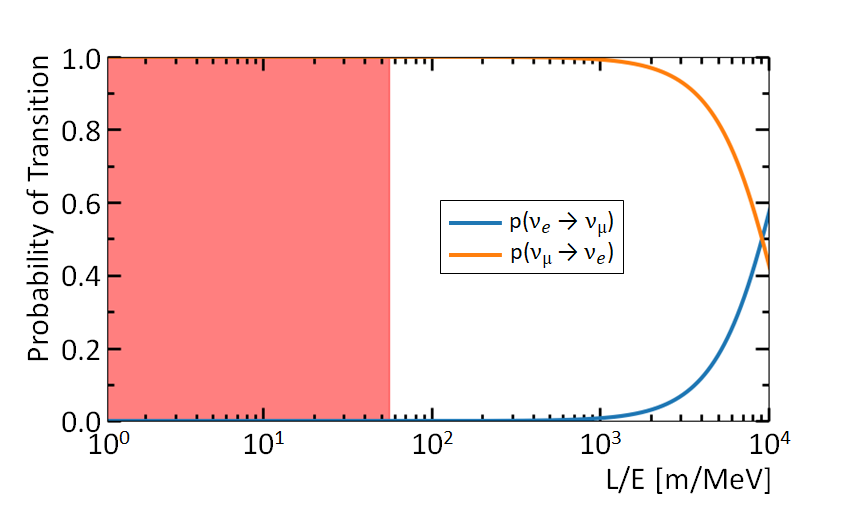
\includegraphics[width=0.8\linewidth]{Chapter2/Figs/neutrinoLOverE_0-2000_ReactorRanges_10-8.5_100-1.8_Log_Adjusted_MedText.png}
  \captionof{figure}{L/E values for the two neutrino case. Assuming near-field ranges between 10\,m -- 100\,m and reactor $\nu$ energies of 1.8\,MeV -- 8.5\,MeV \cite{Mueller_2011} L/E values of 1.18\,m/MeV -- 55.6\,m/MeV are produced and shown via the highlighted area. In the highlighted area there is no significant probability of standard neutrino oscillation.}%The L/E values for neutrino transition for a two neutrino case. The highlighted area represents reactor neutrinos assuming a minimum detectable neutrino energy of 1.8\,MeV and maximum of 8.5\,MeV for reactors \cite{Mueller_2011}. Near-field reactor monitoring distances are assumed to vary between 10\,m to 100\,m. This leads to a minimum L/E of 10\,m/8.5\,MeV = 1.18\,m/MeV and a maximum L/E of 100\,m/1.8\,MeV = 55.6\,m/MeV. The expected range for neutrino oscillation is significantly above the reactor monitoring range and as such typical neutrino oscillations will not be a significant effect for near-field reactor monitoring between 10\,m -- 100\,m.}
\label{fig:probabilityNeutrinoTransition}
\end{figure}

%white space
\vspace{5cm}

\section{Mixing Angles}
% Firstly it would be a good idea to pull from \cite{griffiths2008neutrinoOscillations} which does mention that according to equations \ref{linear_combination_eq_9} and \ref{linear_combination_eq_9} the masses must be unequal and cannot be zero. i.e. $m_i \neq m_j$ and $\Delta m_\theta \neq 0$. \\
% The review of particle physics 2014 is probably quite useful here\cite{Olive_2014}, this may also start to bleed into the other sections, results from T2K, dayabay, double CHOOZ and KamLand may need to be added here. As this is quite a difficult section, lot of potential pit falls and I need to make sure the info I give is up to date because the information is changing frequently. 
% \\I need to show the neutrino mixing matrix and how the dirac and Majorana components work with the mixing angles as shown below (the PMNS matrix) 
% \begin{equation}
% U
%     =
%     \begin{bmatrix}
%         c_{12}c_{13} & s_{12}c_{13} & s_{13}e^{-i\delta}\\
%         -s_{12}c_{23} - c_{12}s_{23}s_{13}e^{i\delta} & c_{12}c_{23} - s_{12}s_{23}s_{13}e^{i\delta} & s_{23}c_{13} \\
%         s_{12}s_{23} - c_{12}c_{23}s_{13}e^{i\delta} & -c_{12}s_{23} - s_{12}c_{23}s_{13}e^{i\delta} & c_{23}c_{13} 
%     \end{bmatrix}
%     \\ \times \text{diag}(1, e^{\frac{i\alpha21}{2}} , e^{\frac{i\alpha31}{2}})
%     \label{neutrino_mixing_matrix}
% \end{equation}
% The dirac CP violation phases are represented by the $\delta$ components the Majorana CP violation is represented by the $\alpha$ components this was taken from \cite{Olive_2014}, which extrapolated it from \cite{Bilenky_1980}, \cite{Schechter_and_Valle_1980} both of which are heavily cited articles themselves.It may be a good idea to mention the CKM quark mixing matrix too. and also cite it. 
% \\I also need to cite double chooz whilst \cite{Olive_2014} has a good handle on $\theta_{12}$ (solar) and $\theta_{23}$ (atmosphere) the value of $\theta_{13}$ (reactor) was before the latest results of the double chooz experiments. So I need to hunt down there most recent paper of which I found was \cite{abe2014improved}, but that was in 2014... It is also worth pointing out as \cite{Olive_2014} does that the oscillations for neutrinos will be very different to the oscillations that quarks undergo these mixing angles are very different. Also worth pointing out that so far no evidence for Majorana neutrinos has be found. Mention neutrino-less double beta decay as a possibility for Majorana neutrinos or at least an exclusion of dirac neutrinos \cite{Schechter_and_Valle_1982}. latest. 
According to equations \ref{linear_combination_eq_9} -- \ref{equ:pmuToPe} for oscillations to occur there must be mass differences between the two neutrino types. If neutrinos were massless then the oscillations could not occur as the values for the probabilities would be zero according to equations \ref{linear_combination_eq_9} -- \ref{equ:pmuToPe}. Therefore, the existence of neutrino oscillations shows that the assumption of massless neutrinos is incorrect \cite{griffiths2008neutrinoOscillations} \cite{sassaroli1999neutrino}. It is assumed that the neutrino flavours follow lepton flavour giving: $\nu_e$, $\nu_\mu$, and $\nu_\tau$. The flavor eigenstates dictate neutrino interactions, but neutrinos propagate as flavor eigenstates of the free-particle Hamiltonian - the mass eigenstates $\nu_1$, $\nu_2$ and $\nu_3$. The flavour mass eigenstates evolve complexly due to the three different masses contributing to the pattern   \cite{griffiths2008neutrinoOscillations}. 
\\\\These flavour changes can be represented by three different angles $\theta_{12}$ ($\theta_{sol}$), $\theta_{23}$ ($\theta_{atm}$), $\theta_{13}$ ($\theta_{reactor}$) \cite{Olive_2014}  \cite{griffiths2008neutrinoOscillations}. These angles can be represented by the following  matrix in equation \ref{PMNS_matrix} which is referred to as the Pontecorvo–Maki–Nakagawa–Sakata (PMNS) matrix.
\begin{equation}
U
    =
    \begin{bmatrix}
        c_{12}c_{13} & s_{12}c_{13} & s_{13}e^{-i\delta}\\
        -s_{12}c_{23} - c_{12}s_{23}s_{13}e^{i\delta} & c_{12}c_{23} - s_{12}s_{23}s_{13}e^{i\delta} & s_{23}c_{13} \\
        s_{12}s_{23} - c_{12}c_{23}s_{13}e^{i\delta} & -c_{12}s_{23} - s_{12}c_{23}s_{13}e^{i\delta} & c_{23}c_{13} 
    \end{bmatrix}
    \\ \times \text{diag}(1, e^{\frac{i\alpha21}{2}} , e^{\frac{i\alpha31}{2}})
    \label{PMNS_matrix}
\end{equation}
Where $s_{ij}$ and $c_{ij}$ represent $\sin(\theta_{ij})$ and $\cos(\theta_{ij})$ respectively. The equation is also parameterized by the CP violation phases $\delta$ and $\alpha$ which represent the Dirac and Majorana phases respectively \cite{Olive_2014}. However, at this time experiments to prove the Majorana over Dirac neutrinos have not proven fruitful as neutrino-less double beta decay has not been observed due to the challenging theoretical and experimental requirements (though experiments are improving their precision) \cite{Cardani_2019}.  So the above PNMS matrix is often written without the Majorana component ($\text{diag}(1, e^{\frac{i\alpha21}{2}} , e^{\frac{i\alpha31}{2}})$). 
\\\\Reducing the errors on the mixing angles has been ongoing effort in neutrino physics. As a result, there are many experiments that have contributed to the improvements in angles which can be seen in figure \ref{neutrino_angles_experiments_variations} 
 which shows the regions favoured or excluded by the oscillation experiments. The measurement of solar neutrinos and the resulting solar neutrino problem has already been covered. And due to the abundance of solar neutrinos the angle $\theta_{12}$ has been measured frequently as seen in figure \ref{neutrino_angles_experiments_variations}. There is also an abundance of terrestrial $\nu_\mu$s which are produced in the atmosphere from cosmic proton interactions which in turn produce $\pi$ which decay into $\mu$ and $\nu_\mu$ \cite{griffiths2008neutrinoOscillations} (see equations \ref{pi_plus_neutrino_production}, \ref{pi_minus_neutrino_production}).
\begin{equation}
    \pi^+ \rightarrow \mu^+ + \nu_\mu,\quad \mu^+ \rightarrow e^+ + \nu_e + \Bar{\nu}_\mu 
    \label{pi_plus_neutrino_production}
\end{equation}
\begin{equation}
    \pi^- \rightarrow \mu^- + \nu_\mu, \quad \mu^- \rightarrow e^- + \nu_e + \Bar{\nu}_\mu 
    \label{pi_minus_neutrino_production}
\end{equation}
\begin{figure}[!h]
 \centering
 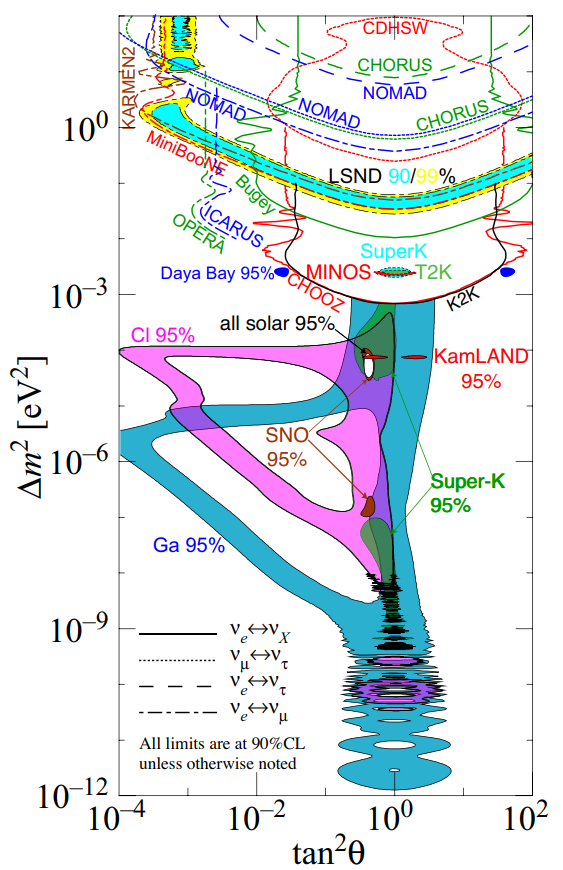
\includegraphics[height=100mm]{Chapter1/Figs/Raster/neutrino_angles_experiments_variations.png} %height of this plot had to be adjusted because of its unusal diemensions
 \captionof{figure}{The regions of squared-mass splitting and mixing angle favoured or excluded by various experiments based on two-flavour neutrino oscillation analyses. From \cite{Olive_2014}.} %~can be used as a kind of place holder in latex
 \label{neutrino_angles_experiments_variations}
\end{figure}
Therefore, there has been an increase in the number of experiments measuring $\theta_{13}$ however due to the production of $\nu_e$s from the sun this presents a unique challenge \cite{Olive_2014}. The solution is to use reactor produced $\Bar{\nu_e}$s at a baseline of $\sim$ 1\,km such that oscillations driven by $\Delta m_{\textrm{sol}}^2$ are negligible. The first experiment to do this was the Chooz experiment, however, it was unable to find any evidence of $\Bar{\nu_e}$ disappearance \cite{Olive_2014}. But the experiment was revised into the Double Chooz experiment which has been able to measure $\Bar{\nu_e}$ disappearance (see section  \ref{subSec:doubleChooz}). These results are also corroborated by RENO (see section \ref{subSec:reno}). The current values are $\sin^2(\theta_{12}) = 0.307 \pm 0.013$, $\sin^2(\theta_{23}) = 0.546 \pm 0.021$, and $\sin^2(\theta_{13}) = 0.0220 \pm 0.0007$ according to the PDG at time of writing \cite{Zyla_pdg_2020}.


\section{Sterile Neutrinos}
%micro boone paper\cite{Karagiorgi_2012}, neutrino 4 paper \cite{neutrino4_2021}, micro boone arxiv for sterile search \cite{denton2021sterile}
Sterile neutrinos are a dark matter candidates that are theorised to potentially occur at short base lines and are currently being investigated using near-field reactor monitoring. Results from Neutrino 4 have suggested sterile neutrino oscillations in the 6\,m -- 12\,m range \cite{neutrino4_2021}. However, considering the recent nature of these results and their lack of replication at time of writing the existence of sterile neutrinos is still hotly debated. Even so, the oscillations proposed are < $\sim$ 10\,m \cite{neutrino4_2021} (see figure \ref{fig:neutrino4Plot}) and so would not be a concern for  VIDARR which will be deployed $\sim$ 50\,m from a reactor. However, it would be possible to mount the VIDARR detector on rails or lorry and attempt to replicate the Neutrino 4 results if shielding was sufficient. 
\\\\In addition, a 100 ton liquid Argon detector called MicroBooNE \cite{Karagiorgi_2012} is currently taking measurements at time of writing. Again preliminary results suggest that sterile neutrinos are plausible but only to within 2.2 $\sigma$ \cite{denton2021sterile}. But these results are from a preprint and so are currently waiting for the rest of the physics community to peer review them. It must be stressed that at present the existence and nature of sterile neutrinos is up for debate. They are included here to show that their proposed nature should not impact reactor monitoring at a distance > $\sim$ 10\,m  where VIDARR will be situated. And that it may be possible to use VIDARR, once it is constructed, to investigate this avenue of new physics.

\begin{figure}[!h]
 \centering
 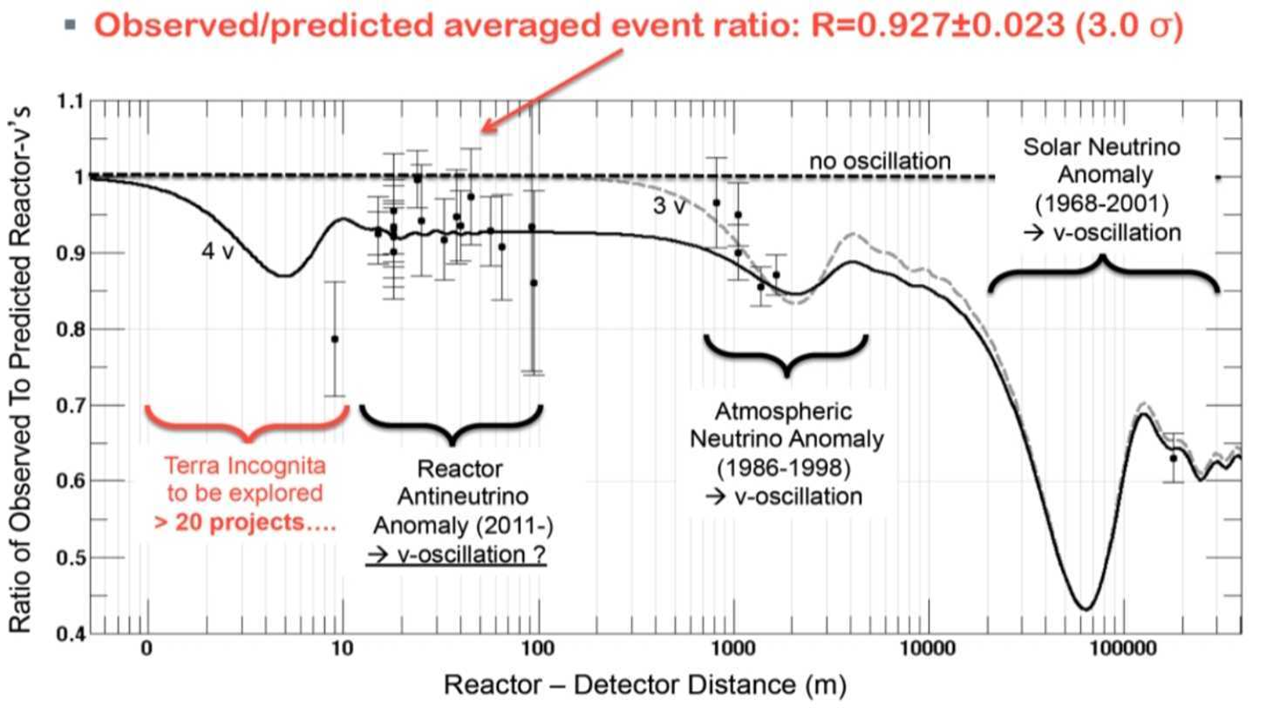
\includegraphics[width=0.8\linewidth]{Chapter2/Figs/neutrino4PlotStretched.jpg}
 \captionof{figure}{The possible process of oscillations to a sterile state at small distances of Neutrino-4 from the active zone of the SM-3 reactor other $\nu_e$ oscillations and anomalies are shown for completeness. From \cite{neutrino4_2021}.} 
 \label{fig:neutrino4Plot}
\end{figure}

%There is also a micro boone internal note that may be of use for sterile neutrinos\cite{microboonecollaboration2021search} 

\section{Reactor Neutrino Anomaly And 5\,MeV ``Shoulder''}
% In figure \ref{fig:neutrino4Plot} between 10\,m -- 100\,m there is an area dedicated to the reactor neutrino anomaly. This anomaly was \cite{mention_anAnomaly_2011}, 
% \\\\(papers: double chooz paper \cite{Abe_2012}, reno paper \cite{reno_may_2012}, Daya Bay paper \cite{dayaBay2016_anFlux}, rmills paper \cite{Hayes_implicationsShoulder_2015}, neutron energies on fission spectra \cite{littleJohn_fissionAnSpectra_2018}, Revealing fine an structure from a reactor \cite{AaSonzogni_fineAnSpectra_2017}, microBoone serach \cite{microboonecollaboration2021search}, \cite{Ashenfelter_PROSPECT_2016}).  
Modelling reactor neutrinos is also an active field of research. There are multiple data bases that describe neutrino energies. For example there are the Huber-Muller, Huber-Haag, JEFF-3.1.1, and ENDF/B-VII.1 spectra \cite{Hayes_implicationsShoulder_2015}. These spectra and others like them help to produce an expected neutrino rate. The expected neutrino theory/data ratio should be $\sim 1$, but it is not. Figure \ref{fig:neutrino4Plot} shows between the range from 10\,m -- 100\,m the expected neutrino averaged rate is 0.927 $\pm$ 0.023 to within $3 \sigma$ \cite{neutrino4_2021}. This is the ongoing ``Reactor Neutrino Anomaly'' \cite{mention_anAnomaly_2011}.  This anomaly is possible evidence for a fourth sterile neutrino \cite{mention_anAnomaly_2011}. But considering that the anomaly maybe due to incomplete modelling it is not definitive proof. %But the existence of sterile neutrinos is still awaiting conformation and replication at time of writing.
\\\\In addition, there is the 5\,MeV ``shoulder'' or ``bump.'' This ``bump'' is an excess at $\sim$ 5\,MeV in the measured reactor neutrino rates as shown by figure \ref{fig:5MevBumps_DB_R_DC}. This 5\,MeV bump was shown by the Daya-bay collaboration by $\sim 4 \sigma$ in the 4\,MeV -- 6\,MeV range when comparing to the Huber-Muller spectrum \cite{dayaBay2016_anFlux} (see figure \ref{subFig:DayaBay5MevBump}) this bump is also clearly seen by the  RENO collaboration (figure \ref{subFig:Reno5MevBump}) \cite{Hayes_implicationsShoulder_2015} \cite{dayaBay2016_anFlux} \cite{reno_recentResults_2014}. Although the Double Chooz comparison (figure \ref{subFig:DoubleChooz5MevBump}) is less pronounced depending on the chosen data base \cite{Hayes_implicationsShoulder_2015}. It has been suggested that deviations in the anti-neutrino spectrum could be caused by decay of certain nuclei (namely $^{95}\textrm{Y}$, $^{98,101}\textrm{Nb}$ and $^{102}\textrm{Tc}$). But to test this hypothesis a new generation of detectors such as PROSPECT \cite{Ashenfelter_PROSPECT_2016} will be required. As they will allow for 0.1\,MeV binning or less as opposed to the current 0.25\,MeV binning (i.e better energy resolution) \cite{AaSonzogni_fineAnSpectra_2017}. Both of these effects will have an impact on the results of VIDARR as the detector will likely be deployed at $\sim$ 50\,m from the reactor core. The observed/predicted neutrino rate is expected to be $\sim$ 0.93 of what the current reactor models suggest and there will likely be a bump at 5\,MeV in the data sets when compared to current reactor models. These effects will likely be in any reactor spectra that VIDARR measures and as they are expected the impact should be minimal or accounted for.

\begin{figure}[!h]
\centering
\begin{subfigure}{.48\textwidth}
  \centering
  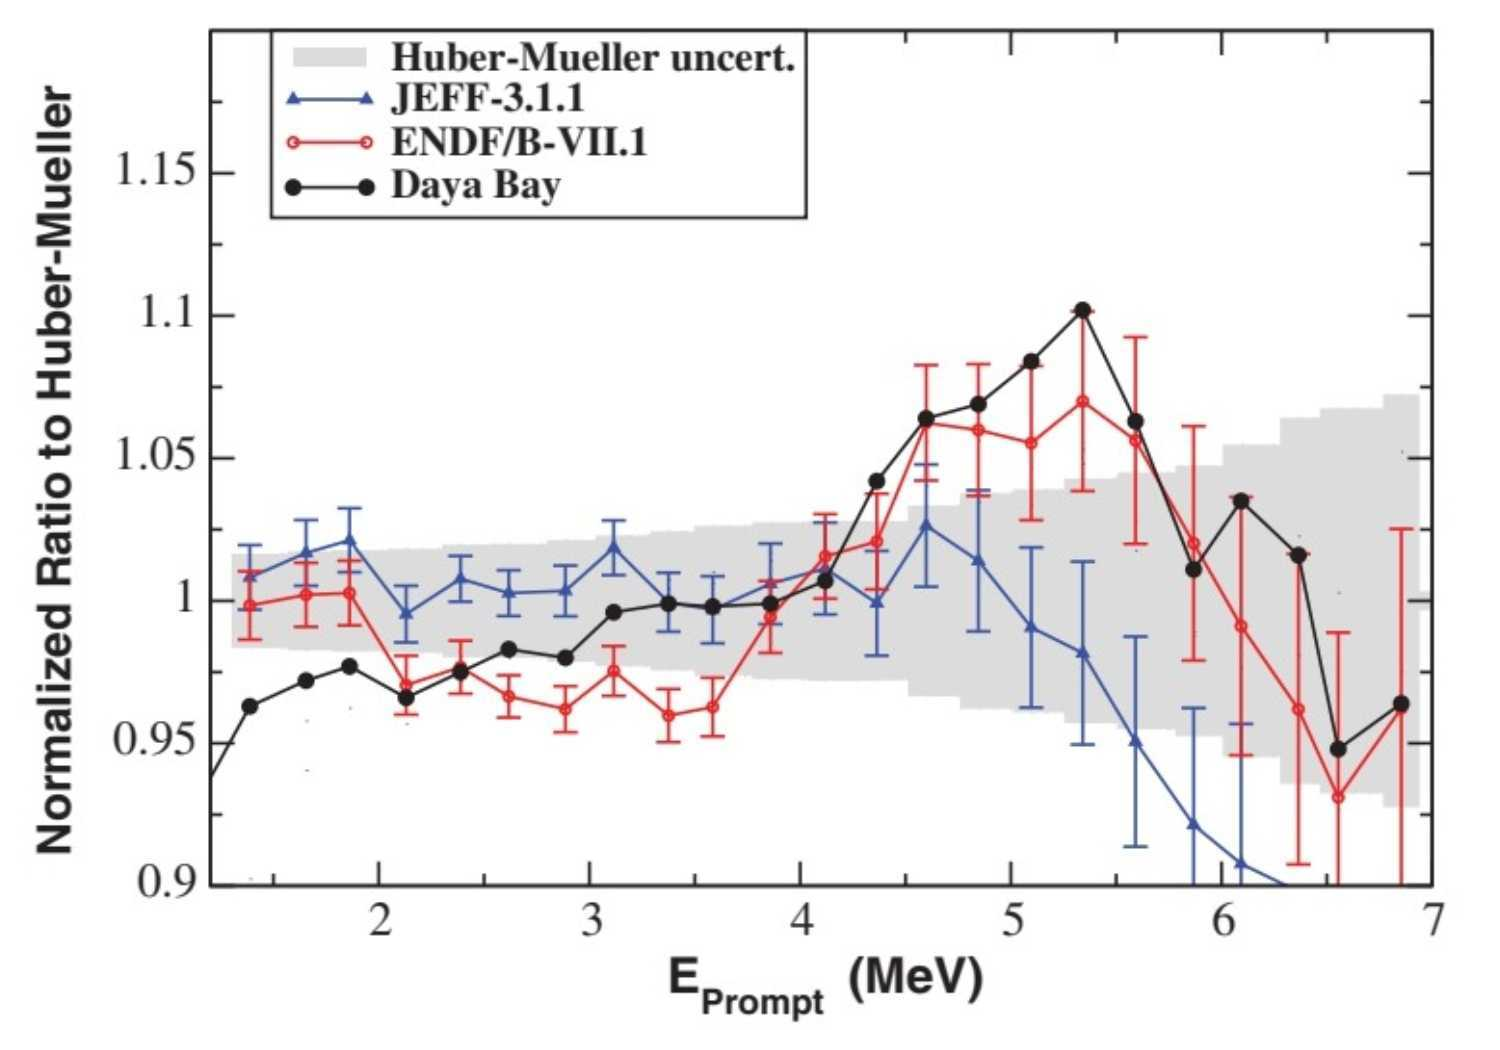
\includegraphics[width=\linewidth]{Chapter2/Figs/Raster/huberMueller_DayaBay_Rmills2015.png}
  \captionsetup{width=.9\linewidth}
  \caption{}
  \label{subFig:DayaBay5MevBump}
\end{subfigure}%
\begin{subfigure}{.48\textwidth}
  \centering
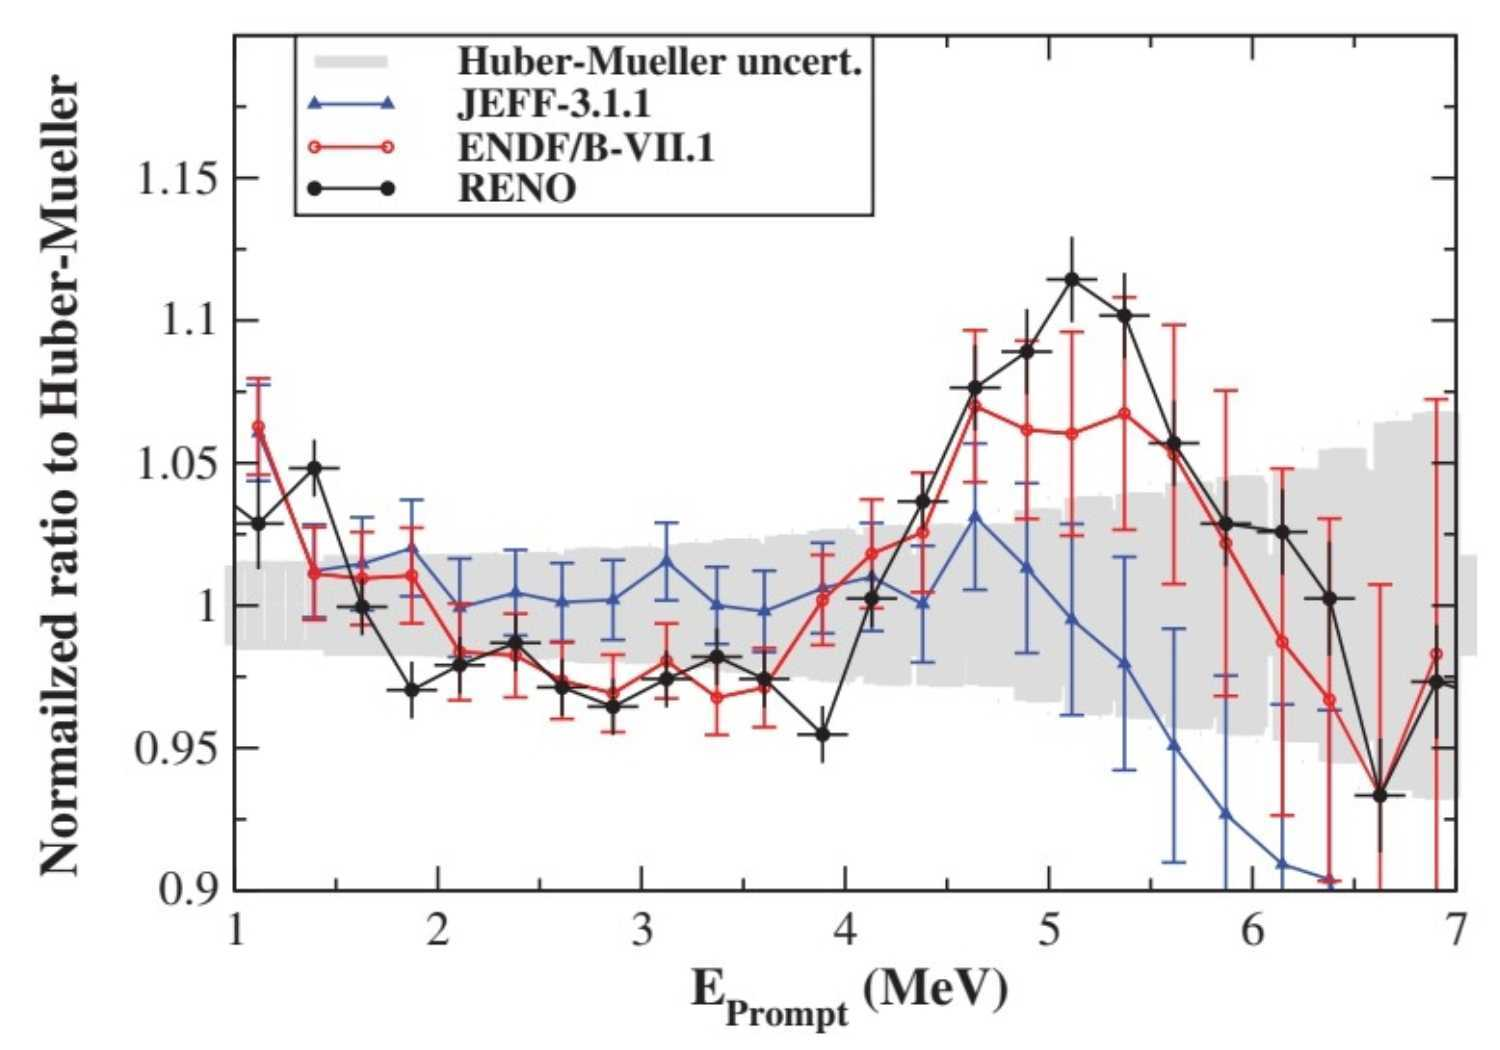
\includegraphics[width=\linewidth]{Chapter2/Figs/Raster/huberMueller_Reno_Rmills2015.png}
  \captionsetup{width=.9\linewidth}
  \caption{}
  \label{subFig:Reno5MevBump}
\end{subfigure}
\begin{subfigure}{.48\textwidth}
  \centering
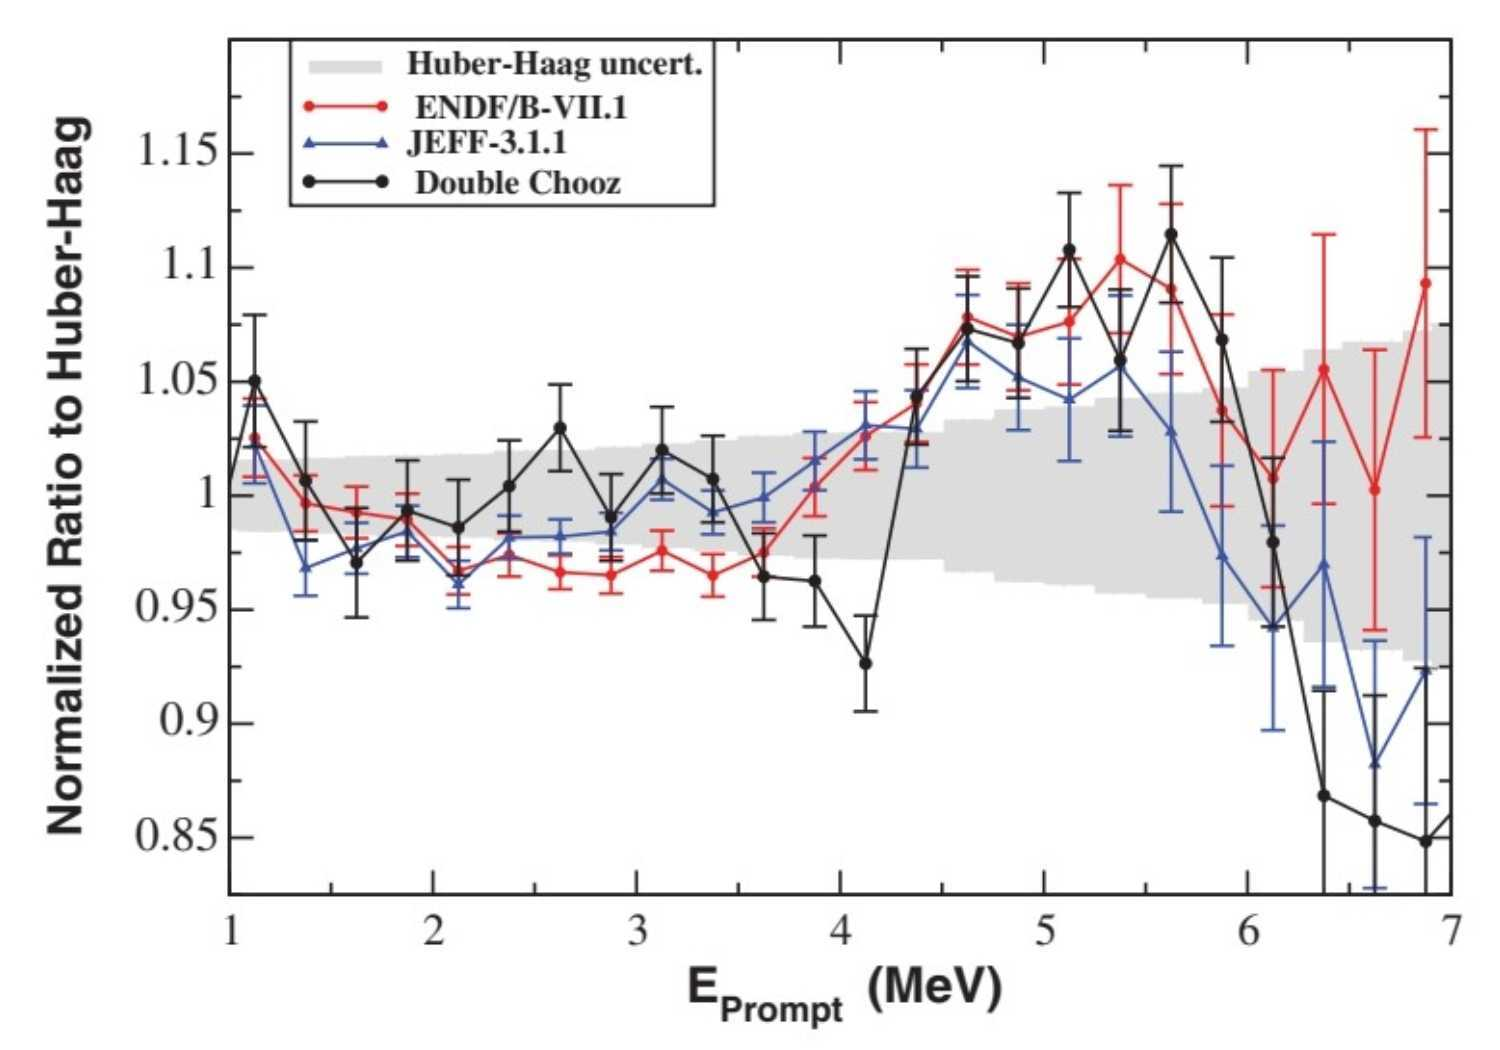
\includegraphics[width=\linewidth]{Chapter2/Figs/Raster/huberHaag_DoubleChooz_Rmills2015.png}
  \captionsetup{width=.9\linewidth}
  \caption{}
  \label{subFig:DoubleChooz5MevBump}
\end{subfigure}
\caption{The 5\,MeV ``shoulder'' for differing experiments. In (a) the Huber-Mueller spectrum is compared to the Daya Bay results \cite{dayaBay2016_anFlux}. In (b) the Huber-Mueller spectrum is compared to the RENO results \cite{reno_recentResults_2014}. In (c) the Huber-Haag spectrum is compared to the Double Chooz results \cite{abe2014improved}. In all cases a clear peak at 5\,MeV can be seen. However, differing data bases such as JEFF-3.1.1 and ENDF/B-VII.1 can exacerbate or flatten the peak. These are in the window $E_\nu$ = 2--8\,MeV ($E_\nu \approx E_{\textrm{prompt}}$ + 0.782\,MeV). From  \cite{Hayes_implicationsShoulder_2015}.}
\label{fig:5MevBumps_DB_R_DC}
\end{figure} 
